%%%%%%%%%%%%%%%%%%%%%%%%%%%%%%%%%%%%%%%%%%%%%%%%%%%%%
%%% Task 4 %%%%%%%%%%%%%%%%%%%%%%%%%%%%%%%%%%%%%%%%%%
%%%%%%%%%%%%%%%%%%%%%%%%%%%%%%%%%%%%%%%%%%%%%%%%%%%%%
\task{Steady-state operation curves of an induction machine}
%%%%%%%%%%%%%%%%%%%%%%%%%%%%%%%%%%%%%%%%%%%%%%
\taskGerman{Betriebskennlinien der Asynchronmaschine}
%%%%%%%%%%%%%%%%%%%%%%%%%%%%%%%%%%%%%%%%%%%%%%

The paramters of a six-pole three-phase induction machine are shown in \autoref{tab:para_inductionMachine}. The nominal stator current is given with $I_{\mathrm{s,n}} = \SI{22.5}{\ampere}$ at a power factor of $\cos(\varphi_{\mathrm{n}})$ = 0.8.

\begin{germanblock}
Die Parameter einer sechspoligen, dreiphasigen Asynchronmaschine sind in \autoref{tab:para_inductionMachine} zu sehen. Der Statornennstrom ist gegeben mit $I_{\mathrm{s,n}} = \SI{22,5}{\ampere}$, bei einem Leistungsfaktor von $\cos(\varphi_{\mathrm{n}})$ = 0.8.    
\end{germanblock}

\begin{table}[htb]
    \caption{Parameters of the induction machine.}
    \centering
    \begin{tabular}{llllll}\toprule
    Symbol       & Value    & Symbol    & Value & Symbol    & Value \\
    \midrule
    $P_{\mathrm{me,n}}$    & $\SI{11}{\kilo\watt}$ & $U_{\mathrm{n}}$   & $\SI{400}{\volt}$ &
    $f_{\mathrm{s,n}}$       & $\SI{50}{\hertz}$       \\ $s_{\mathrm{n}}$    & 0.0444 &
    $R_{\mathrm{s}}$       & $\SI{0.42}{\Omega}$    & $R_{\mathrm{r}}'$    & $\SI{0.459}{\Omega}$ \\
    $L_{\mathrm{\sigma,s}}$  & $\SI{5.1}{\milli\henry}$  & $L_{\mathrm{\sigma,r}}'$    & $\SI{2.4}{\milli\henry}$ &
    $M$ & $\SI{53.2}{\milli\henry}$ \\
    \bottomrule
    \end{tabular}
    \label{tab:para_inductionMachine}
\end{table}
\vspace{-1.3em}
\subtask{Calculate the nominal rotational speed $n_{\mathrm{n}}$ and the nominal torque $T_{\mathrm{n}}$. }{2}
\subtaskGerman{Berechne die nominelle Drehzahl $n_{\mathrm{n}}$ und das Nenndrehmoment $T_{\mathrm{n}}$. }

\begin{solutionblock}
    The nominal rotor frequency is determined by
    $$ f_{\mathrm{r,n}} = \frac{(1-s_{\mathrm{n}})f_{\mathrm{s}}}{p} = \frac{(1-0.0444)\cdot\SI{50}{\hertz}}{3} = \SI{15.93}{\per\second},$$
    which leads to the nominal rotational speed of $\SI{955.6}{\per\minute}$. Hence, the nominal torque is given by:
    $$ T_{\mathrm{n}} = \frac{P_{\mathrm{me,n}}}{\omega_{\mathrm{r,n}}} = \frac{\SI{11}{\kilo\watt}}{\SI{2\pi\cdot 15.93}{\per\second}} = \SI{109.9}{\newton\metre}.$$
    
\end{solutionblock}


\subtask{Calculate the nominal electrical power $P_{\mathrm{el,n}}$ and the efficiency $\eta_{\mathrm{n}}$.}{2}
\subtaskGerman{Berechnen Sie die nominelle elektische Leistung $P_{\mathrm{el,n}}$ und den Wirkungsgrad $\eta_{\mathrm{n}}$.}

\begin{solutionblock}
    The electrical power is calculated by:
    $$ P_{\mathrm{el,n}} = 3 U_{\mathrm{s}} I_{\mathrm{s,n}} \cos(\varphi_{\mathrm{n}}) = 3 \frac{U_{\mathrm{n}}}{\sqrt{3}} I_{\mathrm{s,n}} \cos(\varphi_{\mathrm{n}}) =  3 \cdot \frac{\SI{400}{\volt}}{\sqrt{3}} \cdot \SI{22,5}{\ampere} \cdot 0.8 = \SI{12471}{\watt}.$$

    Moreover, the efficiency is determined as follows:
    $$ \eta_{\mathrm{n}} = \frac{P_{\mathrm{me,n}}}{P_{\mathrm{el,n}}} = \frac{\SI{11000}{\watt}}{\SI{12471}{\watt}} = 0.88.$$

\end{solutionblock}

\subtask{Determine the leakage coefficient $\sigma$.}{1}
\subtaskGerman{Bestimme den Streukoeffizienten $\sigma$.}

\begin{solutionblock}
    The leakage coefficient is determined as:
    \begin{align*}
        \begin{split}
            \sigma &=  1 - \frac{M^2}{\left(M+L_{\mathrm{\sigma,s}}\right)\left(M+L_{\mathrm{\sigma,r}}'\right)} \\
            &= 1 - \frac{\left(\SI{53.2}{\milli\henry}\right)^2}{\left(\SI{53.2}{\milli\henry}+ \SI{5.1}{\milli\henry}\right)\left(\SI{53.2}{\milli\henry}+ \SI{2.4}{\milli\henry}\right)} = 0.13.
        \end{split}
    \end{align*}
\end{solutionblock}

\subtask{Calculate the nominal slip frequency $\omega_{\mathrm{slip}}$ and the maximum angular frequency $\omega_{\mathrm{max}}$.}{2}
\subtaskGerman{Berechne die nominelle Schlupfkreisfrequenz $\omega_{\mathrm{slip}}$ und die maximale Kreisfrequenz $\omega_{\mathrm{max}}$. }

\begin{solutionblock}
    The angular slip frequency is defined by
    $$ \omega_{\mathrm{slip}} = s_{\mathrm{n}} \omega_{\mathrm{s}} = 0.0444 \cdot \SI{2\pi \cdot 50}{\per\second} = \SI{13.95}{\per\second},$$
    and the maximum angular frequency is given with:
    $$ \omega_{\mathrm{max}} = \frac{R_{\mathrm{r}}'}{\sigma \left(L_{\mathrm{\sigma,r}}' + M\right)} = \frac{\SI{0.459}{\Omega}}{0.13\cdot \left(\SI{2.4}{\milli\henry} + \SI{53.2}{\milli\henry}\right)} = \SI{65.3}{\per\second}. $$

\end{solutionblock}

\subtask{Determine the torque and mechanical power for different slip ratios and use these support points to draw the torque and power curves in \autoref{fig:task_T_P}.}{4}
\begin{hintblock}
    The torque equation is given with: $T = T_{\mathrm{max}} \frac{2}{\frac{s}{s_{\mathrm{max}}}+ \frac{s_{\mathrm{max}}}{s}}$.
\end{hintblock}
\subtaskGerman{Bestimmen Sie das Drehmoment und die mech. Leistung für verschiedene Schlupfverhältnisses. Verwenden Sie diese Stützpunkte, um die Drehmoment- und Leistungskurven in \autoref{fig:task_T_P} zu ergänzen.}
\begin{germanhintblock}
    Die Drehmomentgleichung ist gegeben mit: $T = T_{\mathrm{max}} \frac{2}{\frac{s}{s_{\mathrm{max}}}+ \frac{s_{\mathrm{max}}}{s}}$.
\end{germanhintblock}

\begin{figure}[htb]
    \centering
    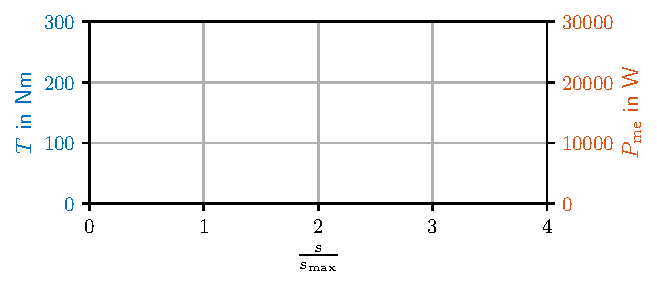
\includegraphics{fig/task_T_P.pdf}
    \caption{Given template to draw the curves for the torque and mechanical power.}
    \label{fig:task_T_P}
\end{figure}

\begin{solutionblock}
    The maximum achievable torque for a constant stator excitation is:
    \begin{align*}
        \begin{split}
            T_{\mathrm{max}} &= \frac{3}{2}p \frac{U_{\mathrm{s}}^2}{\omega_{\mathrm{s}}^2} \frac{M^2}{\sigma\left(L_{\sigma,s} + M \right)^2 \left(L_{\mathrm{\sigma,r}}'+M\right)}\\
            &= \frac{3}{2}\cdot 3 \cdot \frac{\left(\SI{\frac{400}{\sqrt{3}}}{\volt}\right)^2}{\left(2\pi\cdot\SI{50}{\per\second}\right)}\cdot \frac{\left(\SI{53.2}{\milli\henry}\right)}{\left(\SI{5.1}{\milli\henry}+ \SI{53.2}{\milli\henry}\right)^2\left(\SI{2.4}{\milli\henry}+ \SI{53.2}{\milli\henry}\right)}\\
            &= \SI{287.8}{\newton\metre}.
        \end{split}
    \end{align*} 

    The machine-dependent parameter $s_{\mathrm{max}}$ is given with:
    $$ s_{\mathrm{max}} = \frac{\omega_{\mathrm{max}}}{\omega_{\mathrm{s}}} = \frac{R_{\mathrm{r}}'}{\sigma \left(L_{\mathrm{\sigma,r}}'+ M \right)\omega_{\mathrm{s}}} = \frac{\SI{0.459}{\Omega}}{0.13\cdot \left(\SI{2.4}{\milli\henry} + \SI{53.2}{\milli\henry}\right)\cdot \SI{2\pi\cdot50}{\per\second}} = 0.21. $$

    
    With the utilization of the Kloss's formula, the torque is calculated for given slip ratios, e.g., for $\nicefrac{s}{s_\mathrm{max}} = 2$ as:
    $$ T\left(\frac{s}{s_{\mathrm{max}}}=2\right) = T_{\mathrm{max}} \frac{2}{\frac{s}{s_{\mathrm{max}}} + \frac{s_{\mathrm{max}}}{s}} = \SI{287.8}{\newton\metre}\cdot \frac{2}{2 + \frac{1}{2}} = \SI{230.2}{\newton\metre}. $$

    The mechanical power is given with
    $$ P_{\mathrm{me}} = T \omega_{\mathrm{r}} = T \frac{(1-s)f_{\mathrm{s}}}{p} 2\pi, $$
    and, e.g., for $\nicefrac{s}{s_\mathrm{max}} = 2$ as:
    $$ P_{\mathrm{me}}\left(\frac{s}{s_{\mathrm{max}}}=2\right) = \SI{230.2}{\newton\metre} \cdot \frac{\left(1-2\cdot0.21\right)\cdot \SI{50}{\per\second}}{3} \cdot 2\pi = \SI{13981}{\watt}.$$

    To sketch the torque and mechanical power curves, some support points are calculated, which are shown in \autoref{tab:sol_torque_power}.
    \begin{solutiontable}[htb]
        \centering
        \caption{Calculated torque and mechanical power dependant on the ratio $\nicefrac{s}{s_{\mathrm{max}}}$.}
        \begin{tabular}{cccccc}\toprule
            $\frac{s}{s_{\mathrm{max}}}$ & 0 & 1 & 2 & 3 & 4 \\
            \midrule
            T & 0 & \SI{287.8}{\newton\metre} & \SI{230.2}{\newton\metre} & \SI{172.7}{\newton\metre} & \SI{135.4}{\newton\metre}\\
            $P_{\mathrm{me}}$ & 0 & \SI{23809}{\watt} & \SI{13981}{\watt} & \SI{6691}{\watt} & \SI{2267}{\watt} \\
            \bottomrule
        \end{tabular}
        \label{tab:sol_torque_power}
    \end{solutiontable}

    Hence, the resulting trajectories are shown in \autoref{fig:sol_T_P}.
    \begin{solutionfigure}[htb]
        \centering
        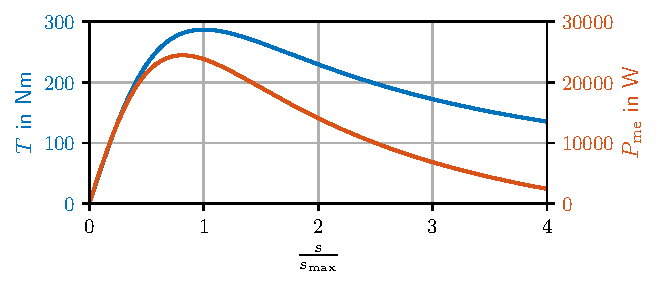
\includegraphics{fig/sol_T_P.pdf}
        \caption{Trajectory of the torque and mechanical power.}
        \label{fig:sol_T_P}
    \end{solutionfigure}


\end{solutionblock}


\subtask{Is the mechanical power zero for a theoretical consideration of an infinitely large mechanical speed (negative and positive speed values)?}{2}
\subtaskGerman{Ist die mechanische Leistung im theoretischen Grenzfall unendlich hoher positiver oder unendlich negativer Drehzahl Null?}

\begin{solutionblock}
    The mechanical power is given with
    $$ P_{\mathrm{me}} = T \omega_{\mathrm{r}}, $$

    considering the given hint results into:
    $$ P_{\mathrm{me}} = T_{\mathrm{max}} \frac{2}{\frac{s}{s_{\mathrm{max}}}+ \frac{s_{\mathrm{max}}}{s}} \frac{(1-s)f_{\mathrm{s}}}{p} 2\pi. $$

    The power for an infinite high or low rotational speed is given as:
    $$ \lim_{s \to \pm \infty} P_{\mathrm{me}} = -T_{\mathrm{max}} \frac{2}{\frac{1}{s_{\mathrm{max}}}} \frac{f_{\mathrm{s}}}{p}2\pi = -\SI{287.8}{\newton\metre} \cdot \frac{2}{\frac{1}{0.21}} \cdot \frac{\SI{50}{\per\second}}{3}\cdot 2\pi = \SI{-12658}{\watt}. $$ 
    
\end{solutionblock}






